\documentclass[a4paper]{article}

\usepackage[14pt]{extsizes}
\usepackage[T2A]{fontenc}
\usepackage[russian]{babel}

\usepackage[left=20mm, top=15mm, right=15mm, bottom=20mm]{geometry}
\usepackage{listings}
\usepackage{xcolor}
\usepackage{tikz}
\usetikzlibrary{shapes.geometric, arrows.meta, positioning, calc, arrows, shapes.misc}
\usepackage{graphicx}
\usepackage{amsmath, amssymb} % For equations
\usepackage{booktabs} % For better tables
\usepackage{pgfplots} % For plotting graphs
\usepackage{caption} % For captioning tables and figures
\usepackage{float} % For precise float placement (images, tables)
\usepackage[hidelinks]{hyperref} % For table of contents to be clickable
\usepackage{bookmark}
\usepackage{multirow}
\usepackage{array}
\usepackage{cancel}
\usepackage{placeins}
\usepackage{enumitem}
\pgfplotsset{compat=1.17}
\usepackage{circuitikz}
\usetikzlibrary{decorations.markings} % For custom arrow positioning

% -----------------------------------------------------

\newcommand{\labtitle}[9]{
	\begin{center}
		\vspace*{-1.8cm}
		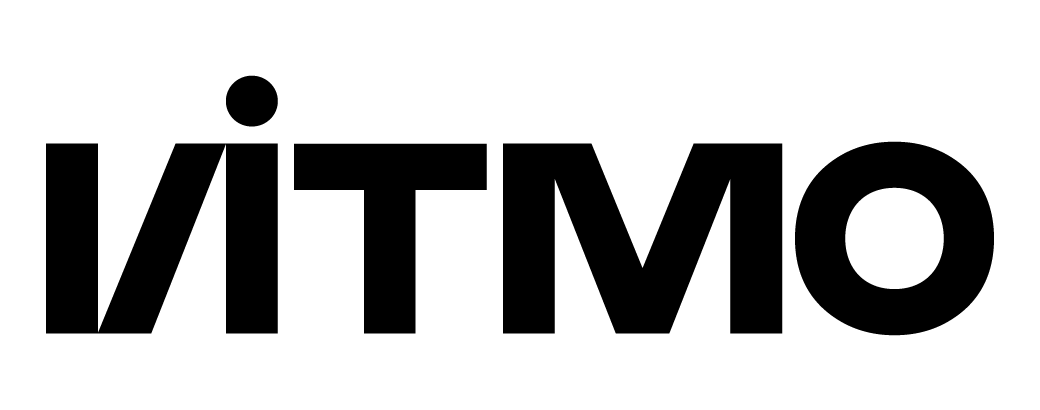
\includegraphics[width=0.26\textwidth]{../common/itmo-logo.png}\\
		\vspace{2.4cm}
		\textbf{\Large Основы электротехники}\\[1.2cm]
		\textbf{\Large Отчёт по лабораторной работе №#1}\\[0.7cm]
		\textbf{\Large #2}\\[3cm]

		\textbf{\Large Группа \textcolor{red}{\textit{P#3}}}\\[0.2cm]
		\textbf{\Large Вариант \textcolor{red}{\textit{#4}}}\\[3cm]

		\begin{flushleft}
			\textbf{\large Выполнил: \textcolor{red}{\textit{#5}}}\\[0.5cm]
			\textbf{\large Дата сдачи отчёта: \textcolor{red}{#6}}\\[0.5cm]
			\textbf{\large Дата защиты: \textcolor{red}{#7}}\\[0.5cm]
			\textbf{\large Контрольный срок защиты: \uline{#8}}\\[0.5cm]
			\textbf{\large Количество баллов: \uline{#9}}\\[2cm]
		\end{flushleft}
	\end{center}

	\vspace*{\fill}
	\begin{center}
		\textbf{\Large СПб -- 2024}
	\end{center}
	\vspace*{-1.8cm}
}

\newcommand{\hwtitle}[8]{
	\begin{center}
		\vspace*{-1.8cm}
		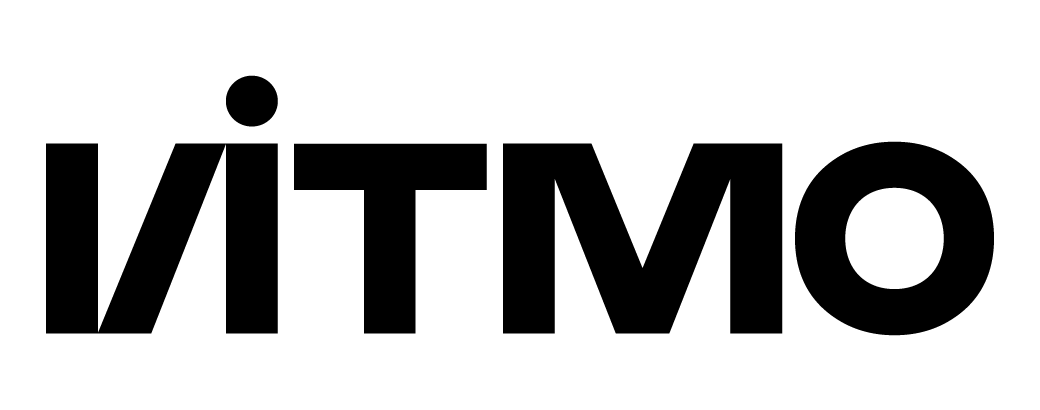
\includegraphics[width=0.26\textwidth]{../common/itmo-logo.png}\\
		\vspace{2.4cm}
		\textbf{\Large Основы электротехники}\\[1.2cm]
		\textbf{\Large Домашнее задание №#1}\\[0.7cm]
		\textbf{\Large #2}\\[3cm]

		\textbf{\Large Группа \textcolor{red}{\textit{P#3}}}\\[0.2cm]
		\textbf{\Large Вариант \textcolor{red}{\textit{#4}}}\\[3cm]

		\begin{flushleft}
			\textbf{\large Выполнил: \textcolor{red}{\textit{#5}}}\\[0.5cm]
			\textbf{\large Дата сдачи: \textcolor{red}{#6}}\\[0.5cm]
			\textbf{\large Контрольный срок сдачи: \uline{#7}}\\[0.5cm]
			\textbf{\large Количество баллов: \uline{#8}}\\[2cm]
		\end{flushleft}
	\end{center}

	\vspace*{\fill}
	\begin{center}
		\textbf{\Large СПб -- 2024}
	\end{center}
	\vspace*{-1.8cm}
}

% % listing for programming code blocks
\lstset{
	language=C++,                 % Programming language
	basicstyle=\ttfamily\normalsize, % Adjust font size
	keywordstyle=\color{blue},    % Style for keywords
	stringstyle=\color{red},      % Style for strings
	commentstyle=\color{gray},   % Style for comments
	morecomment=[l][\color{magenta}]{\#}, % Special comment style
	breaklines=true,              % Line breaking in long lines
	numbers=left,                 % Line numbering on the left
	numberstyle=\tiny\color{gray},% Style for line numbers
	frame=single,                 % Code frame
	showstringspaces=false        % Don't show spaces in strings
}

% % tikz styles for flowcharts
\tikzset{
	startstop/.style={
			rectangle,
			rounded corners,
			minimum width=3cm,
			minimum height=1cm,
			text centered,
			draw=black,
			fill=red!30
		},
	io/.style={
			trapezium,
			trapezium left angle=70,
			trapezium right angle=110,
			minimum width=3cm,
			minimum height=1cm,
			text centered,
			draw=black,
			fill=blue!30
		},
	process/.style={
			rectangle,
			minimum width=3cm,
			minimum height=1cm,
			text centered,
			draw=black,
			fill=orange!30
		},
	decision/.style={
			diamond,
			aspect=2,
			minimum width=3cm,
			text centered,
			draw=black,
			fill=green!30
		},
	arrow/.style={
			thick,
			->,
			>=stealth
		},
	prep/.style={
			chamfered rectangle,
			chamfered rectangle xsep=2cm,
			draw,
			thick,
			minimum width=5cm,
			minimum height=1cm,
			text centered,
			text width=2.5cm,
			font=\small,
			fill=yellow!30
		},
}


\begin{document}

% Title page

% -- choose which one you need --

% laboratory work title
\labtitle{1}{Исследование характеристик источника электрической энергии постоянного тока}{3331}{33}{Дворкин Борис Александрович}{xx.xx.2024}{xx.xx.2024}{09.10.2024}{}
\thispagestyle{empty}

% homework title
\hwtitle{1}{Расчёт цепей постоянного тока}{3331}{33}{Дворкин Борис Александрович}{xx.xx.2024}{04.12.2024}{}
\thispagestyle{empty}

% old basic group lab title
\begin{center}
	\vspace{1cm}
	\large{Университет ИТМО}\\
	\large{Факультет программной инженерии и компьютерной техники}\\
	\vspace{4cm}
	\Large{\textbf{Лабораторная работа №1\\}}
	\vspace{0.3cm}
	\large{\textbf{<<Введение в проектирование цифровых интегральных схем>>\\}}
	\vspace{-0.3cm}
	\begin{center}
		\large{по дисциплине <<Функциональная схемотехника>>}
	\end{center}
	\vspace{3cm}
\end{center}
\normalsize{
	\begin{flushright}
		Выполнили:
		\par
		Студенты группы P3331
		\par
		Дворкин Борис Александрович
		\par
		Краков Кирилл Константинович
		\par
		\textbf{Вариант: 1}
		\par
		\vspace{1cm}
		Преподаватель:
		\par
		Васильев Сергей Евгеньевич
	\end{flushright}
}\\
\vspace{6cm}
\begin{center} г. Санкт-Петербург
	\par
	2024 г.
\end{center}


% old basic group uir title
\begin{center}
	\vspace{1cm}
	\large{Университет ИТМО}\\
	\large{Факультет программной инженерии и компьютерной техники}\\
	\vspace{4cm}
	\Large{\textbf{Учебно-исследовательская работа №1 (УИР 1)\\}}
	\vspace{0.3cm}
	\large{\textbf{<<Кодирование данных в телекоммуникационных системах>>\\}}
	\vspace{-0.3cm}
	\begin{center}
		\large{по дисциплине <<Телекоммуникационные системы>>}
	\end{center}
	\vspace{3cm}
\end{center}
\normalsize{
	\begin{flushright}
		Выполнил:
		\par
		Студент 3 курса группы P3331
		\par
		Дворкин Борис Александрович
		\par
		\textbf{Вариант: ДвБА}
		\par
		\vspace{1cm}
		Преподаватель:
		\par
		Алиеф Тауфик Измайлович
		\par
		\noindent Отчёт принят «\underline{\hspace{0.7cm}}» \underline{\hspace{1.3cm}} 2024 г.\\
		Оценка: \underline{\hspace{2cm}}
	\end{flushright}
}\\
\vspace{6cm}
\begin{center} г. Санкт-Петербург
	\par
	2024 г.
\end{center}
\thispagestyle{empty}
\thispagestyle{empty}


% -------------------------------

\newpage
\pagestyle{plain}
\setcounter{page}{1} % Enable text numbering

% -------------------------------

% autogenerated table of contents
\linespread{0.9}
\tableofcontents
\linespread{1}

% -------------------------------

\newpage
\section*{Цель работы}
\addcontentsline{toc}{section}{Цель работы}

Исследование ... ... ...
% -------------------------------

\section*{Часть 1}
\addcontentsline{toc}{section}{Часть 1}
\stepcounter{section}
% \input{part1}

% -------------------------------

% Other main content
% \input{chart}
% \input{code}
% \input{examples}
% \input{conclusion}

\end{document}
